\documentclass[crop,tikz]{standalone}
\usepackage{tikz}
\usepackage{sfmath}
\renewcommand{\familydefault}{\sfdefault}
\usepackage{pgfplots}
\usepgfplotslibrary{colorbrewer,patchplots}
\pgfplotsset{compat=1.18}
\renewcommand{\vec}{\mathbf}
\begin{document}
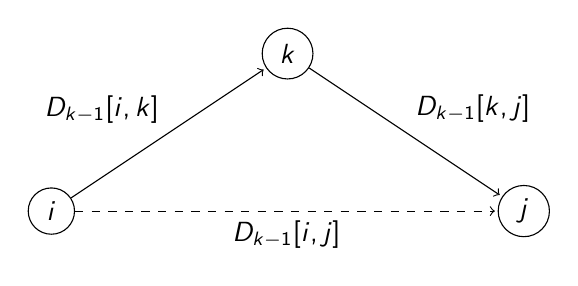
\begin{tikzpicture}[shorten >=1pt,->, vertex/.style = {draw, circle}]
    \node[vertex] (Vi) at (-3, 0) {\(i\)};
    \node[vertex] (Vj) at (3, 0) {\(j\)};
    \node[vertex] (Vk) at (0, 2) {\(k\)};

    \draw[->] (Vi) -- node[above left] {$D_{k-1}[i,k]$} (Vk);
    \draw[->] (Vk) -- node[above right] {$D_{k-1}[k,j]$} (Vj);
    \draw[->, dashed] (Vi) -- node[below] {$D_{k-1}[i,j]$} (Vj);
\end{tikzpicture}
\end{document}